%TODO : cf NOTES.md
%Notes : check biblio, watch out for dates
%Coherence du style : oops WE …
%Attention EXAPTATION
%Cool pour truc “paradoxal” : ++ si DP – ===> lie a ce pb d’honnete…

%BRUIT D’EXPLORATION…
%= critique … 

%Argumenter que binaire mais pas du a artefact pour autant : perspectives…

%- partie 2 spécifier lhusgoire p/np pour : en fait 1.3.6=> truc continu. .. avec à la marge traîtres (comme premier modèle...)
%Mais => Pb de Learning...
%=> Decoupages : bon ba tant qu'à faire binaire

%Puis à la fin : version 2... (Cf part 3) où JB disparaît / histoire change

%Pour demo ss2: check gintis + ...

%TODO : REFERENCES -> citation type = ?
\documentclass[a4paper,12pt]{report}
\usepackage{graphicx}
\usepackage{subcaption}
\usepackage{amsmath}
\usepackage[bottom]{footmisc}
\usepackage{apacite}
\usepackage{pdfpages}
%\usepackage[nottoc]{tocbibind}
%\usepackage{biblatex}
\usepackage[T1]{fontenc}
\usepackage{chngcntr}
\counterwithout{equation}{chapter} % 
\counterwithout{table}{chapter}
\counterwithout{figure}{chapter} % remove chapter number

\usepackage{titlesec, blindtext, color}
\definecolor{gray75}{gray}{0.75}
\newcommand{\hsp}{\hspace{20pt}}
\titleformat{\chapter}[hang]{\Huge\bfseries}{\thechapter\hsp\textcolor{gray75}{|}\hsp}{0pt}{\Huge\bfseries}

\begin{document}

\setlength{\parindent}{0pt}
\setlength{\parskip}{6pt}

\begin{titlepage}
	\centering
    
\includegraphics[width=0.25\textwidth]{cogmaster}\par\vspace{1cm}
    %moche
	{\scshape\LARGE Cogmaster \par}
	\vspace{1cm}
	{\scshape\Large Second-year internship Memoir\par}
	\vspace{1.5cm}
	{\huge\bfseries Self-sacrifice as a social signal\par}
	\vspace{2cm}
	{\Large\itshape Julien Lie\par}
	\vfill
	supervised by\par
	Jean-Louis \textsc{Dessalles}

	\vfill

% Bottom of the page
	{\large \today\par}
\end{titlepage}



\pagenumbering{roman}\tableofcontents\newpage\pagenumbering{arabic}

\part{Declaration of originality}
%% FAIRE DES PDF aussi x2...
- Déclaration d'originalité
Les stages de M2 Recherche doivent être de véritables travaux de recherche originale, pouvant aller au-delà des connaissances déjà publiées (sans préjuger des résultats obtenus). Afin de clarifier cet aspect, chaque étudiant doit faire figurer, en première page de son mémoire, une déclaration d'originalité spécifiant en quoi le travail présenté va au-delà de ce qui est déjà connu.

    pour les travaux expérimentaux
        préciser en quoi les expériences effectuées diffèrent de celles déjà publiées, et en quoi elles pourraient potentiellement permettre de contribuer à résoudre une question non encore élucidée (sans préjuger des résultats obtenus)
    pour les travaux théoriques
        préciser en quoi les idées, modèles ou théories proposés vont au-delà de ceux qui sont publiés, et ont éventuellement un pouvoir explicatif supérieur
    pour les recherches appliquées
        préciser en quoi le dispositif (programme, méthode, traitement, etc.) diffère des dispositifs existants et en quoi ses performances sont potentiellement supérieures

\part{Declaration of contribution}
- Déclaration de contribution
Comme la plupart des recherches scientifiques, les stages de M2 Recherche impliquent souvent de multiples contributeurs: l'étudiant, l'encadrant, mais souvent aussi d'autres membres du laboratoire qui aident à des titres divers. Il s'agit de préciser, comme dans un nombre croissant de revues, les contributions respectives de toutes ces personnes. A cet effet, chaque étudiant doit faire figurer, en première page de son mémoire, une déclaration de contribution, qui précise de manière nominative toutes les personnes qui ont contribué à:

        la définition de la question scientifique qui est posée
        la recherche bibliographique permettant de cerner la question et de guider le choix de l'approche et de la méthodologie
        le choix de l'approche générale pour répondre à la question
        le choix de la méthodologie spécifique
        la mise au point de la méthodologie
        la programmation de l'expérience ou du modèle
        le recrutement des sujets
        le test des sujets
        le dépouillement, le codage des données
        l'analyse des données
        l'interprétation des résultats et la formulation des conclusions
        la rédaction du mémoire, la production de tables ou de figures
        la relecture et les commentaires sur le mémoire
        etc.

Attention, ces points sont donnés à titre indicatif! Ils ne s'appliquent pas nécessairement à tous les types de projets. La déclaration de contribution doit être rédigée par l’étudiant d’après cette liste indicative.


\part{Pre-registration document}
% A INSERER DIRECT EN PDF SINON RELOU...
% en rajoutant "pre-registration..." ?
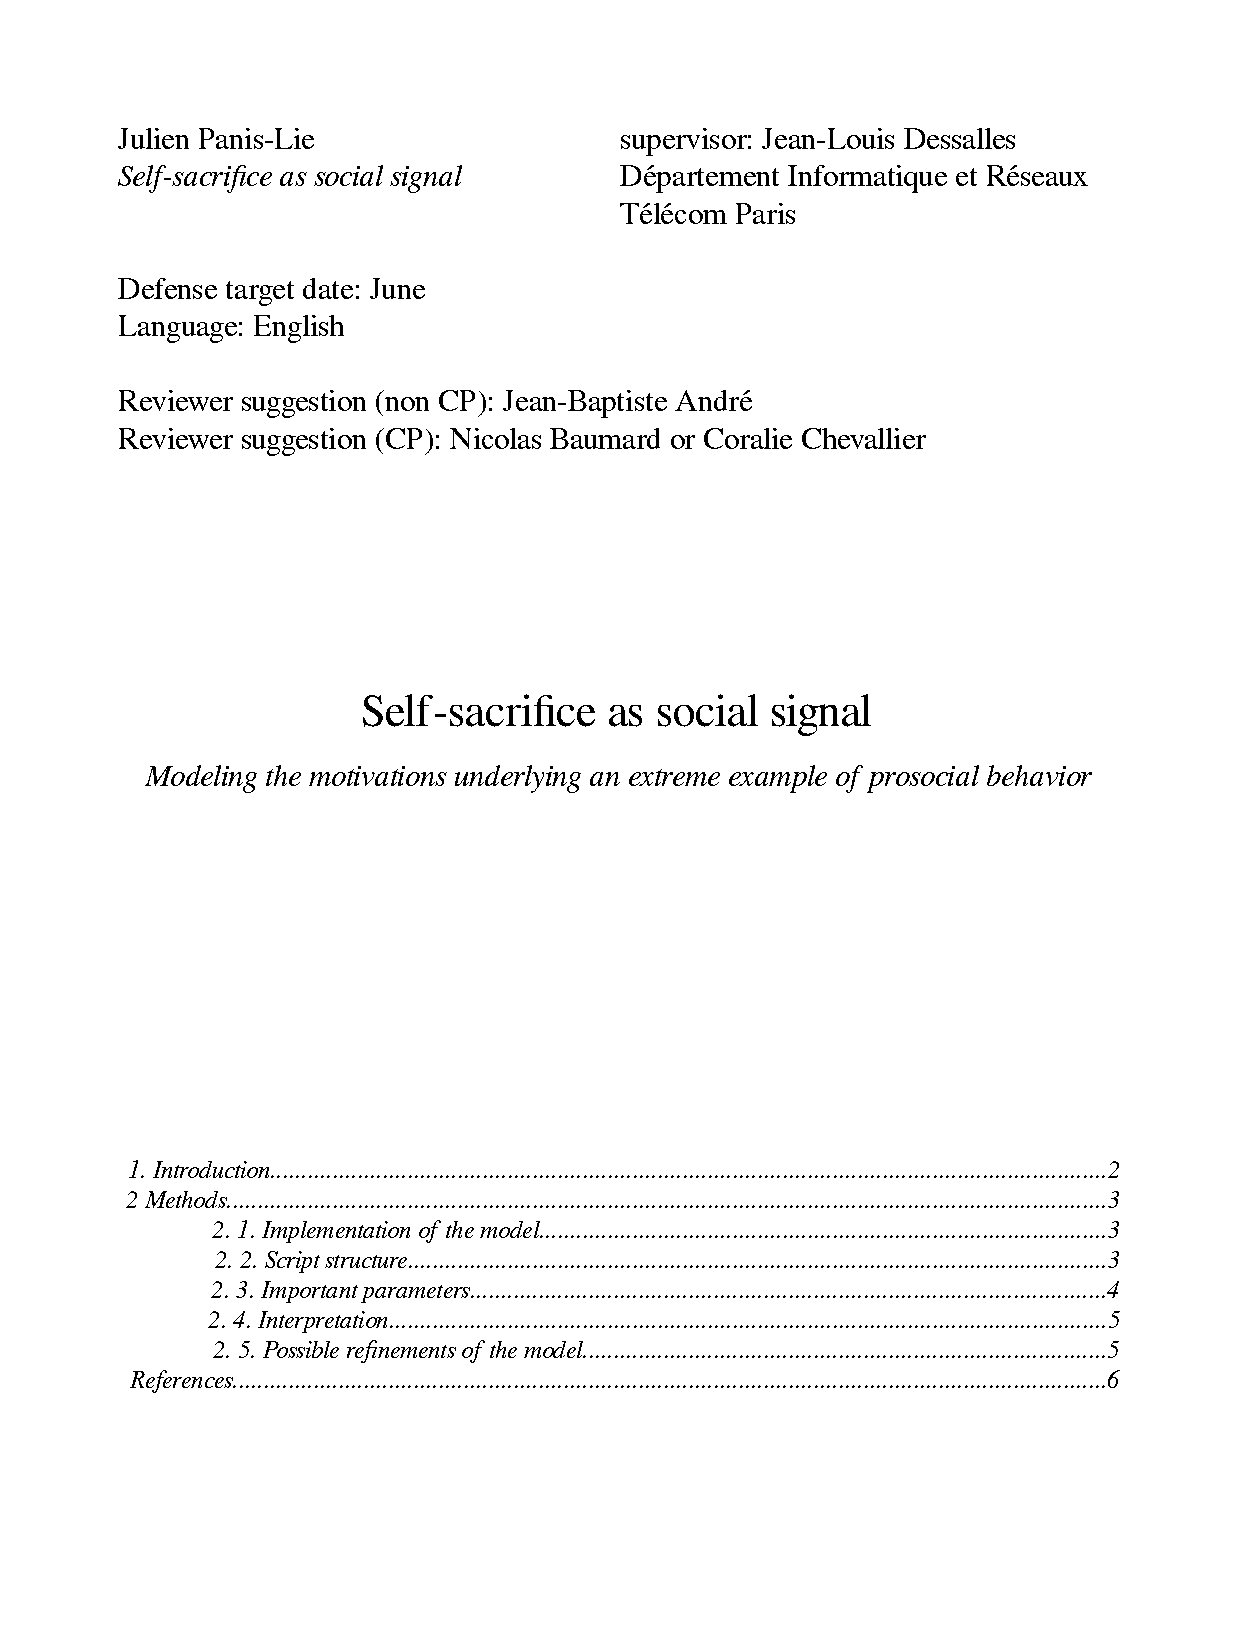
\includepdf[pages=-]{Prereg_v2.pdf}
\part{Self-sacrifice as a social signal}

\chapter{Why do humans self-sacrifice for their groups?}
\section{Self-sacrifice}
\label{s:intro}
\subsection{Prevalence and characteristics of self-sacrifice in humans}
Throughout history, humans have been willing to lay down their lives for the sake of their groups
\cite{whitehouse_dying_2018}.
\citeA[pp. 238-246]{durkheim_suicide:_2007} characterizes such acts as 
“altruistic suicides”,
encompassing any behavior which will \emph{necessarily result in death}, in which individuals engage
knowingly, \emph{in the name of a group and/or its ideology}. Throughout this paper this
will be referred to as extreme \emph{prosocial} self-sacrifice, as it involves extreme costs
to the self (death) intended for the benefit of others – or simply self-sacrifice.

Early Christian martyrs (Durkheim, \emph{ibid}), the 300 Spartans at the Battle of Thermopylae
\cite{lazenby_defence_1993}, kamikaze Japanese pilots during the Second World War and Muslim suicide
terrorists in recent decades \cite{pape_dying_2006} all fall under this definition.

These examples underscore that such self-sacrificial behavior may be related to (perceived)
threat to the group, perhaps notably in a context of intergroup conflict.
Intergroup violence is a widespread and persistent feature of sapiens’ environment
during the Pleistocene, with potentially far-reaching impact on our mortality \cite{keeley_war_1997},
making it likely that mechanisms related to such a situation would have been selected
in our species. 

In contrast however, the sectarians of Amida in the early nineteenth century
(Durkheim, \emph{ibid}) appear to give up their life outside of any such context
\footnote{Although it is hard to rule out (and not specified here) that they
may be motivated by a perceived threat to their sect.}
in \emph{public} displays of piety, their emph{memory} being held in great reverence 
by members of the crowd. Martyrs engaged in intergroup conflict 
also gain posthumous celebrity within the group \cite{blackwell_middle-class_2008}.

\subsection{Identity fusion}
For \citeA{whitehouse_dying_2018}, self-sacrifice for the sake of a group is motivated by
\emph{identity fusion}, a visceral sense of oneness with the group \cite{swann_when_2012}.
Two pathways can lead to enduring identity fusion: perceptions of shared biology, 
or \emph{psychological kinship}, as well as intense collective experiences,
including the horrors of frontline combat or participation in potentially extremely 
\emph{painful rituals}. Highly “fused” individuals appear to take threats
to the group personally, and, in extreme cases, may be motivated to lay down their life
for said group. While the difficulty of evaluating actual would-be martyrs’ motivations
is compounded by practical and ethical issues, one can note that identity fusion is 
correlated with expressions of support for martyrs and even stated willingness to give up one’s 
own life to defend the group \cite{whitehouse_dying_2018}.

Identity fusion accounts for many of the characteristics of self-sacrifice as outlined above,
including its relation to conflict and its stated objective (defense of the group).
In addition, it allows to place willingness to lay down one’s life for a group on a
spectrum and connect it with two other associated social mechanisms – extreme rituals
(e.g. intense initiations, \citeNP[p. 8]{pape_dying_2006}) and metaphors of brotherhood
(or other family-like ties) in public discourse.

Alternative explanations put a more direct emphasis on certain elements evoked above:
ideology \cite{pape_dying_2006}, psychological kinship and social devices that foster perceptions of
familial ties \cite{swann_what_2014}, intense collective experiences and “rites of terror”
\cite{whitehouse_rites_1996} – or, propose that devotion to sacred values \cite{atran_talking_2011} may
also play a causal role.

%Insert figure : Proximate vs ultimate ?

From an evolutionary standpoint however, these explanations only beg the question.
Beliefs, psychological motivations and social mechanisms, whether or not they are
integrated under the concept of identity fusion, are immediate proximate causes for behavior,
which cannot account for the evolution of self-sacrifice in our species \cite{tinbergen_aims_2010}.
At first glance, self-sacrificial behavior and its underlying motivations constitute
a true biological puzzle, since dying is obviously not a good way of passing one one’s genes.
This paper aims to better understand why self-sacrifice, as characterized in these first
two sections exists by taking an evolutionary outlook:

\emph{What are the ultimate causes of self-sacrifice for the sake of the group, 
which may account for the evolution and maintenance of such behavior in humans?}

\section{Existing ultimate (biological) explanations for self-sacrifice}
\label{s:xpla}
Explanations for self-sacrifice usually invoke maladaptive behavior
(pathology, miscalculation…), kin selection or group benefit – or, a mixture of the three.

\subsection{Self-sacrifice does not need (more) explaining}
\label{ss:error}
For some authors, self-sacrifice (particularly in the modern form of suicide terrorism)
is caused by extreme religious views and/or pathology \cite[p. 16]{pape_dying_2006}.
This does not square however with the extent of such behavior, which is also displayed
by individuals one would more intuitively link to patriotic or nationalist beliefs
(Spartians at Thermopylae, kamikaze during World War II).

More importantly, the persistence of self-sacrifice throughout our history suggests
that pathology may not be a sufficient explanation. If self-sacrifice is maladaptive,
seeing its huge costs to individual fitness, \emph{why did such behavior evolve in our species?}
In addition, contemporary studies of individuals who engage in such behavior suggest
they have no appreciable psychopathology and are as educated and well-off as 
surrounding populations \cite{atran_genesis_2003}.

A related argument is that such behavior should not be understood as
functionally self-sacrificial. The biological \emph{function} of a behavior is an effect
of that trait that causally explains its evolution and persistence in a population
\cite{nettle_evolution_2009}.
%or other ref
As outlined in \textbf{Section \ref{s:heroism}}, heroism may have a social function which
allows to account for the evolution of heroic behavior particularly in times of intergroup
conflict. Such heroic behavior may sometimes result in death, manifestly in favor of
the warring group. In such an interpretation, self-sacrifice is thus accidental, and/or
borne from miscalculation \cite{marie_self-sacrifice_2018}.

The distinction between risking one’s life and laying it down is not always clear-cut.
According to one estimate \cite[p. 272]{gambetta_making_2006}, one has only a 1 in 10 chance 
of surviving an act worthy of a British Commonwealth Victoria Cross medal, 
making it hard to decide whether such acts should be characterized as heroic
or self-sacrificial. For cases such as the examples given above,
which involve long-term planning (e.g. Muslim suicide terrorists)
and repetitive actions that can only realistically result in death (e.g. Christian martyrs),
it seems hard to avoid the latter qualification – unless one factors in severe and
dire miscalculation. This explanation is thus similar to the previous “pathological” one;
the same objections can be made.

\subsection{Kin selection}
\label{s:kin}
Throughout the natural world, one example of prosocial behavior abounds: parental care.
Costly behavior in favor of children (and more generally, kin) is adaptive if,
from the standpoint of genes, costs are outweighed by benefits,
as captured by Hamilton’s rule \citeyear{hamilton_genetical_1964}: if costs $c$ associated with a behavior are
smaller than benefits $b$ to a kin times coefficient of genetic relationship $r$,
then, on average, a gene that favors said behavior will leave more copies than a
gene that does not. At the individual level, this is captured by the concept of
\emph{inclusive fitness}.

 \[\textnormal{Hamilton's rule: }b*r > c\]

Hamilton’s rule leaves the door open to even self-sacrificial behavior in favor of kin.
Thus, in some (rare) examples, such as certain spiders \cite{kim_functional_2000},
mothers are systematically eaten by their offspring (and let them do it) at the end of
their incubation period, a behavior which is sufficiently beneficial to the long-term
prospects of the (tens of) individuals in the clutch to have evolved. Beneficiaries
need not be restricted to immediate offspring: certain aphids and other social insects
may “self-explode”, in order to plaster over gaps in the nest (gall) with their body fluid,
to the benefit of the entire colony \cite{kutsukake_exaggeration_2019}.

\begin{figure}[]Kutsukake et al., 2019
    \centering
    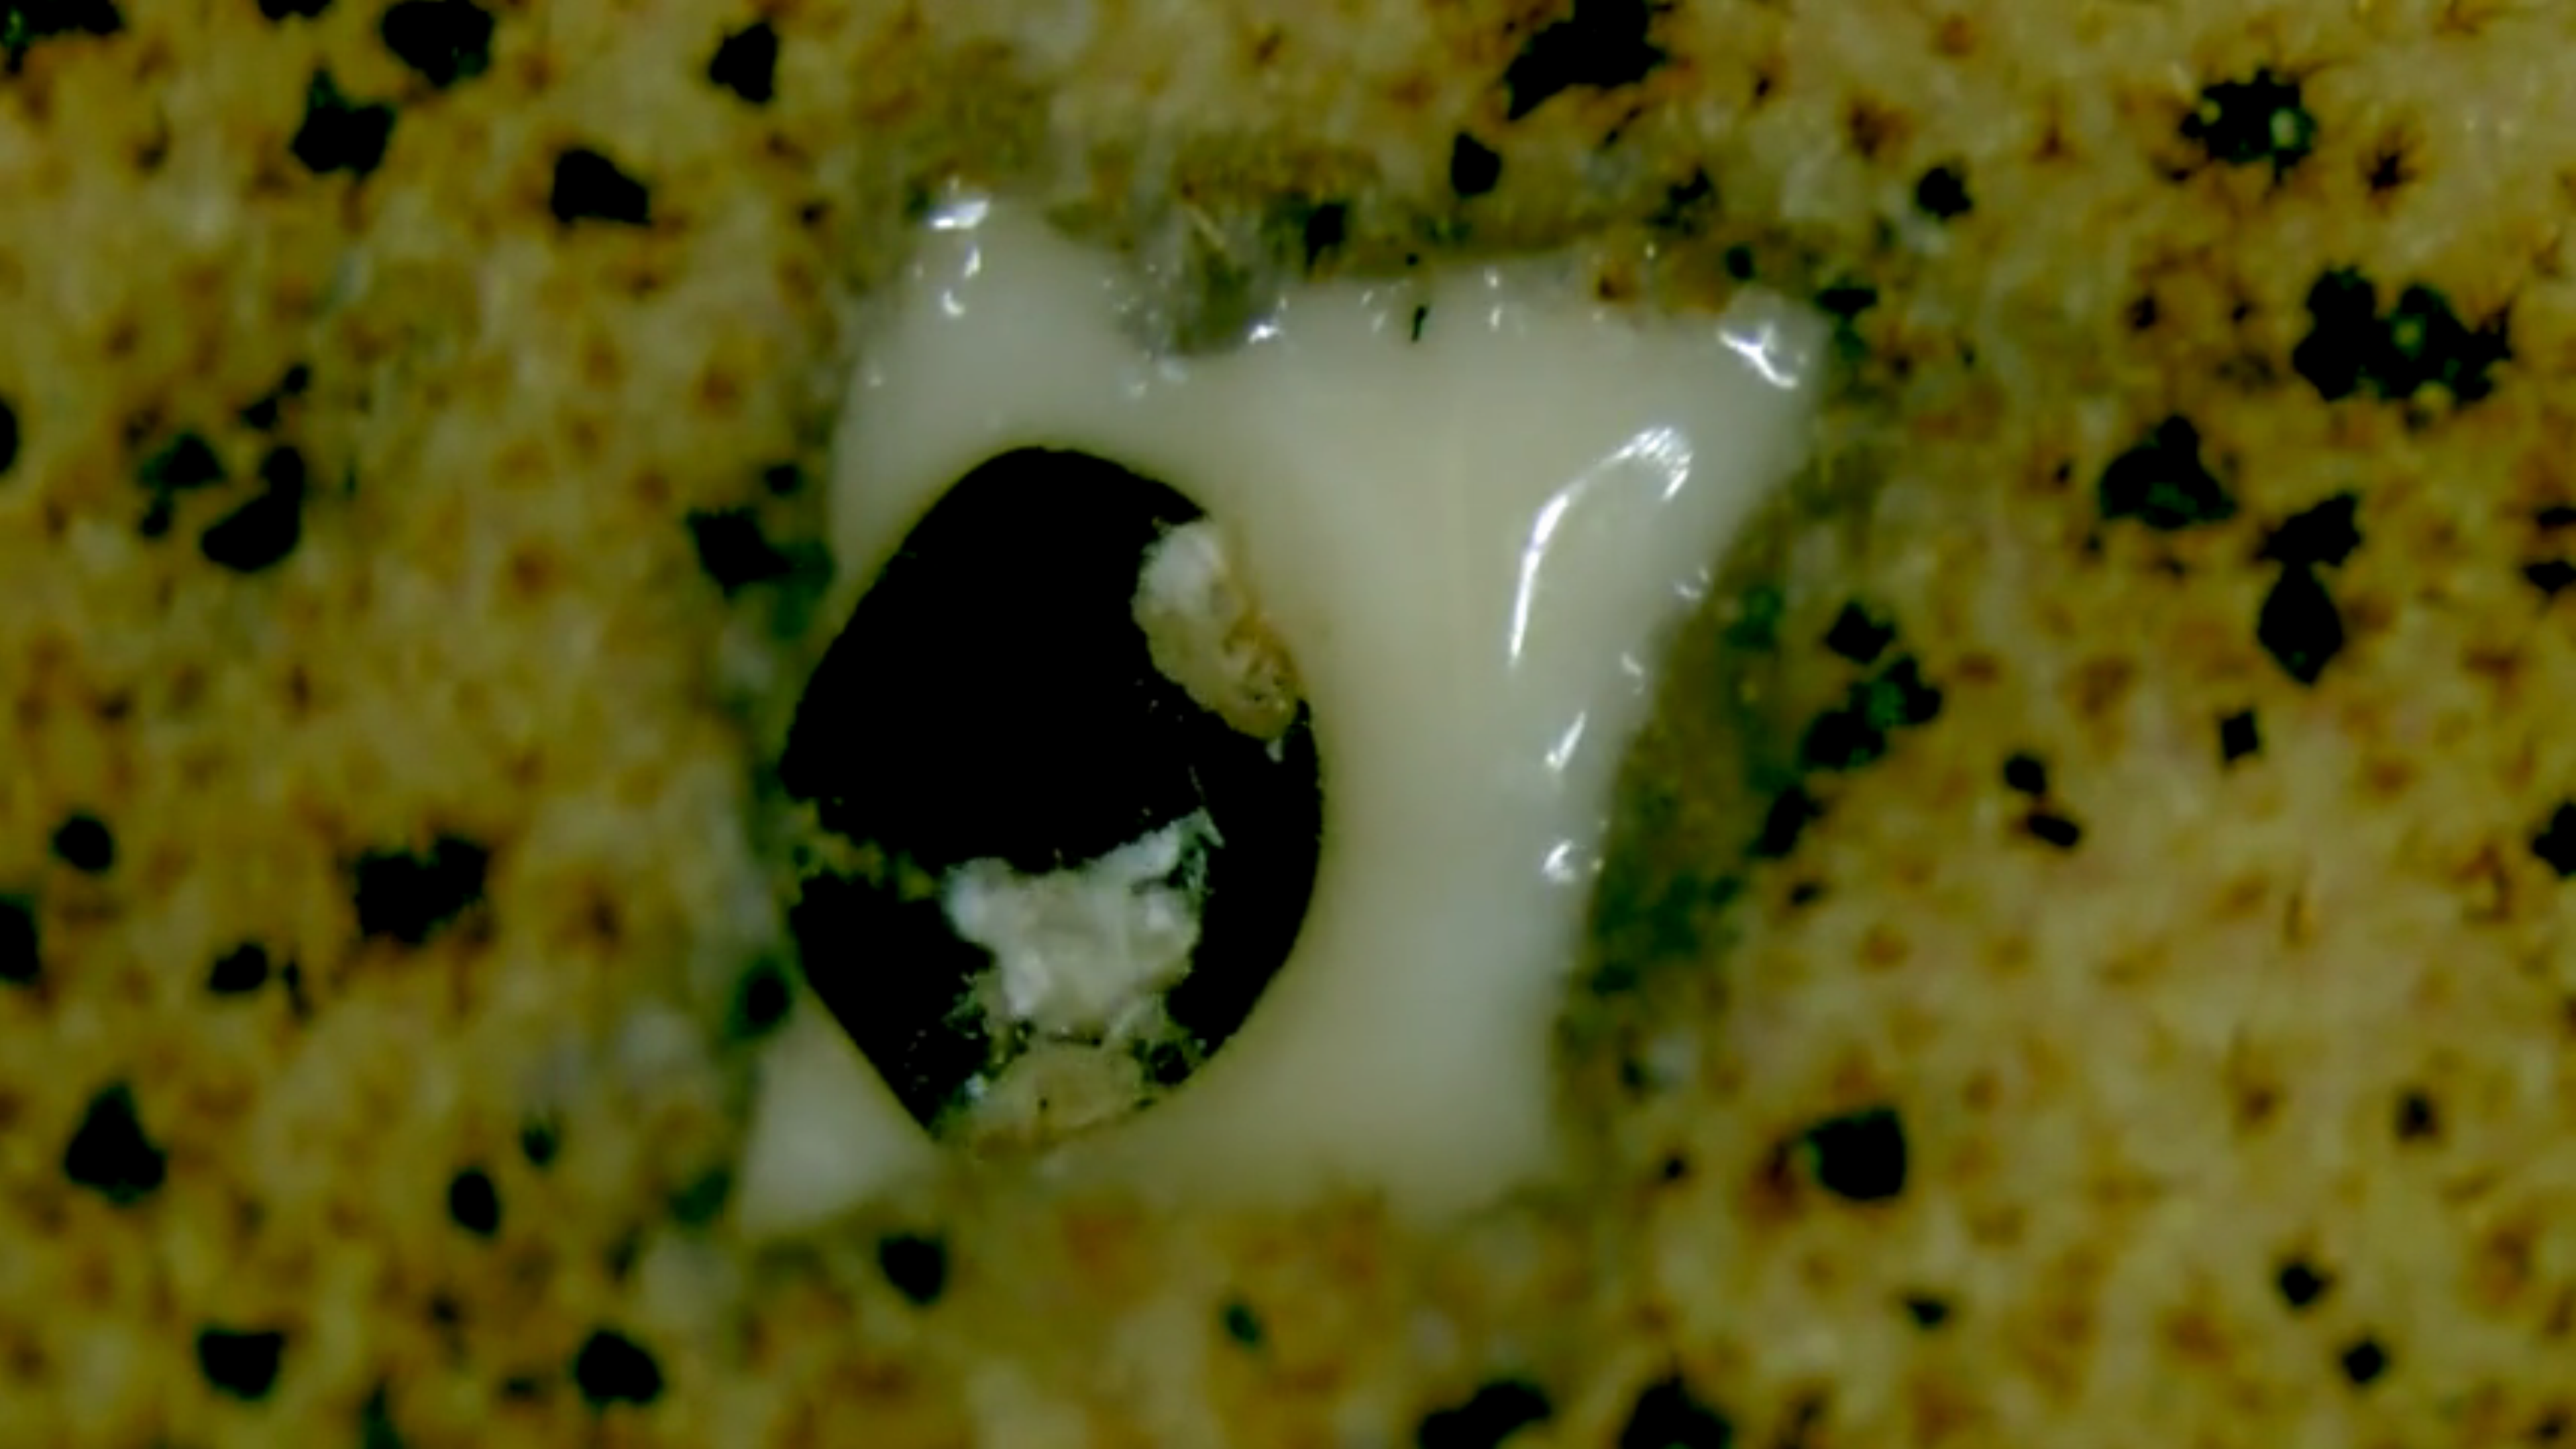
\includegraphics[width=1\textwidth]{aphid}
    \caption{Soldier aphids using their body fluid to repair their gall. Kutsukake et al.,
    via \textit{lemonde.fr}.}
    \label{}
\end{figure}
    
Whitehouse and Lanman \citeyear{whitehouse_ties_2014} argue that kin selection can similarly explain
the evolution and maintenance of identity fusion – and self-sacrifice,
in extreme cases of intergroup conflict. In such an interpretation, 
both pathways leading to fusion (perceived biological relatedness and shared experiences)
and their corresponding social mechanisms (evoking “brotherhood”, rituals…)
come down to the same fundamental issue: detecting your genetic kin, and motivating
potentially extreme behavior in their favor, when the situation demands it (conflict).
This will be referred to as \emph{“kin fusion”}.

Kin fusion rests on the debatable assumption that ancestral warring groups were 
composed of close genetic relatives. Of course, Whitehouse and Lanman do not anticipate
that such genetic proximity should be comparable to that in an aphid gall
\footnote{Contrary to us, social insects reproduce via eusocial division of labor
(a colony descends from one or a small number of “kings” or “queens”) or cloning.
Two random individuals taken in a colony may thus be very closely related (tentatively,
r measurable in tens of percentage points) – considerably more so than
two random hunter-gatherers taken in a typical unit of over 100 individuals \cite{dunbar_grooming_1996}.
If however, on average, these two individuals are significantly more related than
two individuals in two different groups, self-sacrifice may still theoretically emerge,
provided benefits to kin are large enough.},
but merely significant enough for similar kin self-sacrifice to remain a theoretical
possibility. Studies of current hunter-gatherer groups \cite{hill_co-residence_2011} and of fossils
\cite{sikora_ancient_2017} suggest however that ancestral human groups were highly fluid and not
closely related.

%%%%% A reformuler
In any case, even if one accepts that self-sacrifice through fusion may evolved
to favor ancestral groups of kin, the question remains: \emph{why would such behavior be
maintained?} In the historical examples given, groups who are intended to benefit
from self-sacrifice (e.g. national or religious community) are too large to be
genetically related. From an evolutionary standpoint, feeling fused to such a large group
to the point of self-sacrifice thus constitutes an extremely costly mistake –
which brings us back to the arguments developed in the previous section.

%A reformuler selon commentaire/critique d’un ami: c’est pas exactement
%un argument basé sur l’erreur mais sur le concept d’exaptation :
%une adaptation utilisé au-delà de son domaine propre.
%Réponse du coup: oui mais là, le mismatch dure “trop” longtemps
%(contrairement au sucre par exemple). Et les impacts sur la fitness sont énormes
%(au contraire de la reco de visages mignons et de Mickey, par exemple).

Another way of complementing – or replacing – this explanation revolves around group and/or cultural selection, as detailed in the next section. Alternatively, Blackwell (2008) notes that, for Palestinian suicide fighters, self-sacrifice comes with material gains to the family. In certain economic situations, self-sacrifice may thus increase an individual’s inclusive fitness.
This is similar to the arguments developed in \textbf{Section \ref{s:ss_sgl}}, although
Blackwell’s model does not specify how such a situation may come to be.

\subsection{Group benefit; cultural selection}
%Section a retravailler je pense : cf JLD comm
Another family of explanations starts from self-sacrifice’s stated objective:
collective benefit. Groups comprising prosocial individuals should fare better
than groups of egoists at the collective level – offering another perspective on insect
eusociality \cite{nowak_evolution_2010} and human prosocial behavior
\cite{wilson_evolution_2008}.

Many authors object to the idea that natural selection should (also) occur at the
level of the group, as, in practice, human collective dynamics seem not to verify
its axioms (\citeNP{williams_adaptation_1996}; \citeNP{buss_false_2015}).
% Pinker ou Buss apparait ?
They argue that the fundamental level
for natural selection is genetic: what determines the evolution of a heritable behavior
is, all else being equal, the number of copies that genes3 controlling it leave in the
next generation \cite{dawkins_selfish_1976}. Following this view, selection at the individual level
is merely an approximation, which can be made in numerous cases because of how inter-related
the fate of an individual’s genes are – a condition which does not seem to be met at
the collective level4. At the individual level, purely prosocial behavior
(with no supplementary benefit to the individual with respect to others)
is a losing strategy, as illustrated by the tragedy of the commons \cite{hardin_tragedy_1968}
– and should therefore be counter-selected.

In particular, explanations for self-sacrifice in terms of collective benefit make a
questionable assumption: that groups may face threat of complete annihilation.
Orbell and Moriwaka \citeyear{orbell_evolutionary_2011} argue that in such a context, kin fusion could extend to
larger coalitions comprising non-related individuals, while Whitehouse et al. \citeyear{whitehouse_evolution_2017}
content that fusion and self-sacrifice can evolve directly for groups of non-kin,
provided prosocial behavior is conditioned on past shared experiences. Their two-tier
model (individual and group levels) includes the same assumption, as groups performing
badly increase their chances of being completely replaced by the offspring of another
group. Yet, from the standpoint of genes, prehistoric group extinction seems highly
unlikely: even if the entirety of its (predominately male) fighting force is massacred,
civilian women may survive to join other groups and/or be subject to rape, as is
recurrent in such conflicts \cite{gottschall_explaining_2004}.

%%[Figure 4 = probabilite de mort du groupe chez Whitehouse]

Another related explanation revolves around the idea of cultural selection:
that cultural objects may follow a process akin to Darwinian natural selection
\cite{richerson_cultural_2016}. Thus, norms or social institutions may for instance have
evolved to exploit the previously described propensity to fuse and potentially
self-sacrifice for kin (Orbell \& Moriwaka, 2011; Swann et al., 2012; Whitehouse, 2019).
Such an explanation could be more robust to the previous criticism: it may be less
debatable to suggest that norms or institutions can disappear, although this neglects
the fact that such cultural elements cannot exist purely outside of individuals’ minds
\cite{boyer_minds_2018}. As with group selection, many argue that cultural dynamics violate
Darwinian axioms – in particular, cultural transmission seems far from random and
culture does not appear to exhibit inheritance in the strict sense
(\citeNP{sperber_why_2006}; \citeNP{buss_false_2015}).
%Re : buss ou PInker

Additionally, from a purely individual standpoint,
self-sacrifice in response to such a potentially selected norm or institution
remains an evolutionary mistake, as argued above.

\section{Hypothesis: self-sacrifice as a social signal}
\label{s:ss_sgl}
\subsection{Biological signaling}
This question was studied during the internship following a signaling framework.
According to the evolutionary theory of costly signaling \cite{zahavi_mate_1975},
natural selection may, under certain conditions, lead to waste at the individual level
(a handicap). Zahavi’s handicap principle has helped explain counterintuitive phenomenons
across the natural world, from the brightness of male plumage in certain bird species
\cite{zahavi_mate_1975}, which make them more visible to predators, to stotting –
whereby certain preys (e.g. gazelles) will jump up into the air upon predator encounter,
apparently making them easier to catch \cite{maynard_smith_animal_2003}.

A typical signaling model involves senders (signalers) and an audience
(receivers) and can be grounded in evolutionary game theory.
Senders vary in some specific unobservable \emph{quality} of interest to the audience
(note that without variation, there is no need for signals).
They may advertise this quality to their audience, which may infer actual quality
from these signals and base subsequent choices on these inferences
(e.g. mate selection or prey pursuit – see under). Under reasonable mathematical
assumptions
\footnote{Honesty, cost, and increasing cost for males of lesser quality –
as well as more technical elements \cite{grafen_biological_1990}.}
, a signaling equilibrium consisting in a pair of evolutionarily
stable strategies – or ESS \cite{maynard_smith_logic_1973}
%, as introduced by Maynard Smith \citeyear{maynard_smith_evolution_1982}
– for senders and receivers, can be shown to exist \cite{grafen_biological_1990}.
In other words, if one assumes that the strategies followed by senders and receivers
– signaling at a certain level and inferring quality from signals –
are biologically encoded and heritable, then natural selection
can lead to a non-trivial signaling equilibrium which is resistant to
invasion by mutants (alternative strategies).

%Figure 5 : inserer le principe du signal : cf CRI (ou maths Grafen)

Conversely, given such an ESS pair, one can deduce: that signaling should be \emph{honest},
meaning that advertised levels should reflect actual quality; that signalers should
bear a fitness cost (handicap); and that said cost should be higher for senders
of worst quality \cite{grafen_biological_1990}. This is what makes signaling theory so relevant to
ethology: if one observes a situation where individual animals may be understood to
be signaling a quality to an audience, then these signals should be honest and costly
\footnote{If one assumes that signaling level (sender strategy) and inferring quality
from signals (receiver strategy) are biologically encoded and inheritable, 
and therefore subject to natural selection – which converges to ESS equilibria.}.
Honesty is key: if a signal is dishonest, then using it to infer quality would be
sub-optimal – meaning that the corresponding strategy pair cannot be an ESS.
This framework does not therefore apply to cases of dishonest animal communication.
% A revoir avec idee du signal malhonnete finalement ?

Interpreting a seemingly unlikely phenotypic or behavioral outcome in such a context
can thus allow to explain it. Gazelle stotting can for instance be understood
as an honest signal of its ability to outrun an incoming predator:
the higher it jumps, the longer it can be expected to evade a predator –
and it is strategically optimal for predators to decide which prey to attack
(if any) based on how high they jump. With respect to bird plumage, blue plumage
in male grosbeaks \cite{keyser_structurally_2000} has been interpreted as an honest signal directed
at a female audience of potential mates, although it remains unclear which specific quality
is signaled – leaving room for debate. Finding the correct underlying quality associated
to a (potential) signal, as well as its audience, is not usually straightforward,
as decisions such as sexual partner choices involve a variety of overlapping elements
and decisions processing shaped by natural selection – potentially even including
several qualities and corresponding signals \cite{doucet_multiple_2003}.

%Figure 6: gazelle stotting

\subsection{Social signaling and human prosocial behavior}
\label{s:sgl_h}
The theory of costly signaling has also been used by researchers to help shape our
understanding of human behavior, starting with economists. Over a century ago, 
\cite{veblen_theory_1973}
thus framed higher-class luxury consumption and leisure as signals of their status 
and/or wealth. The underlying logic and assumptions of economic signaling theory is 
the same as before (Spence, 1974), with honesty emerging from competition
\footnote{Which is a fundamental element of Darwin’s \citeyear{darwin_origin_2002} theory of natural selection.
Competition between signalers pushes them to signal at higher levels, up to the point where
marginal gains and marginal costs cancel each other out, making their 
signals honest indications of their inner payoff structure – which is determined by their
quality.}
(and differential costs), providing economists with a framework for understanding costly behavior that is not immediately followed by material benefits.
Human prosocial behavior and its underlying motivations can be framed in this light. 
By definition, prosocial motivations push us to act towards the benefit of others, 
thus often paying a cost (time, money…) that is not immediately followed by benefits 
of the same nature. However, prosocial behavior may entail benefits of a social 
nature along the road, which can be captured by the concept of reputation 
\cite{sperber_moral_2012}. This paves the way for explaining certain prosocial 
behaviors and their underlying prosocial motivations, such as equitable sharing 
and equity \cite{debove_evolutionary_2017}.  Costly signals are themselves 
essential building-blocks in our understanding of the emergence of reputation 
and prosocial motivation in a specific context 
\cite{geoffroy_why_2019}.

In the context of the internship, prosocial motivation was approached 
using costly social signals, whose purpose are to broadcast qualities which 
serve as bases for the establishment of social relations. 
Social signals are evolutionarily stable if they are correlated with qualities 
which increase the fitness of members of the audience \cite{dessalles_optimal_2014}.
For instance, if in a certain context such as intergroup conflict, being acquainted 
with brave individuals increases one’s fitness, then such individuals will be in demand,
and displaying signals correlated with courage becomes a valid strategy, up to a certain
cost.

\subsection{Social signaling and high-cost prosocial behavior}
\label{s:heroism}
Signaling competition can have non-linear effects, as individual decisions depend on 
decisions taken by all or several individuals, leading to the emergence of behavior
at the collective level. Thus, unconstrained competition relations typically leads,
at the collective level, to the emergence of a signaling “elite”, which captures the
lion’s share of asymmetrical social affiliations, and a “silent” majority \cite{dessalles_optimal_2014}.
In such a context, individuals who are unable to attain the levels of the elite have
nothing to gain from signaling and should theoretically refrain from doing so
\footnote{Somewhat similarly, gazelles or other prey who are unable to jump high enough
(due to injury, their age…) should refrain from stotting, leading to segregation between
signalers and non-signalers. Collective dynamics matter only however to the extent that
stotting may depend on the behavior of other gazelles (as being the least fit gazelle
in a group should also lead to not signaling), i. e. to 
the extent to which the audience should be understood as other gazelles, not the predator.}.
Real-world examples include the emergence of “saints” in rural Morocco \cite{gellner_saints_2001}
or the emergence of individuals with thousands if not millions of followers inside each
Twitter community \cite{kwak_what_2010}.

%Fig 7: asmetrical signaling => cf Dessalles, 2014

Competition for signaling can therefore lead to extreme costs. In some situations,
bravery may even be signaled by strong risk-seeking behavior – so long as the associated costs (significantly higher death probability) are upset by even higher benefits (related to the social advantages of being a member of the “elite” in this situation). Thus, while bravery may be supported by genuine prosocial motivations (a genuine concern with the benefit of the group, to the point of risking one’s life for it), prosociality and collective benefit should be understood as part of (signaling) bravery, not its explanation (Patton, 1996).
In contrast, when social relations are constrained to be symmetrical,
competition typically leads to generalized signaling, with individuals pairing
up horizontally with individuals of similar quality \cite{chade_sorting_2017}.
In such an example, one would expect benefits, and therefore signaling cost,
to remain manageable. Real-world examples may include friendship, where the
constraining symmetrizing factor is time spent together \cite{dessalles_optimal_2014},
or sexual pairing in grosbeaks and many other bird species, where care for
offspring most often involves both parents \cite{cockburn_prevalence_2006}.
%Fig 8 : symmetrical signaling => Dessalles
%[[[[rmq : Bon on meurt aussi avec le signal de grosbeak… mais bcp moins ??]]]

\subsection{Self-sacrifice: a two-tier social signaling model}
In a context akin to intergroup conflict, one can imagine that commitment to the group
would also be a socially in-demand quality. Betrayal by friends may for instance be a
real possibility: in such a context, choosing friends who will not betray you for the
enemy would be crucial (and correlate with your fitness), paving the way for costly signals
 intended to demonstrate such commitment, associated with achieving higher social status.

This explanation cannot hold for self-sacrifice as defined here, as death has been assumed
to be certain. Costs associated with self-sacrifice are too large; signalers would not
survive to enjoy the advantages of their new status.
Another hypothesis was thus added to the model studied during the internship:
that \emph{social status be in part heritable for our species},
as the high status of an individual can raise that of every member of his or her family
\cite{service_primitive_1962}.  More specifically, in a situation where self-sacrifice can be
understood as a signal of one’s commitment to to group,
with high potential benefits which senders never enjoy,
it is hypothesized that these social benefits should (at least in part)
\emph{spill over} to members of their family.
Seeing the extreme nature of the costs envisioned,
self-sacrifice can only be stable if it remains a low-frequency behavior
(the fewer the heroes, the higher their status), pushing us to relate this
hypothetical signal with unconstrained competition at a \emph{global} level.

At a more \emph{local} level, individuals have an incentive to advertise their commitment
to the group in a less costly way, in order to form more symmetrical friendship bonds,
as explained above. The idea is that for such individuals, the self-sacrifice of a group
“hero” may constitute an opportunity: if such behavior is understood globally as
demonstrative of commitment to the group, then costly behavior associated to a hero’s
self-sacrifice may also be interpreted as such by potential friends.
Thus, at a local level, individuals may signal their commitment
to the group by \emph{honoring} such fallen heroes, for instance
by engaging in conspicuous ceremonies in their name, in order to attract friends.

If and when honoring emerges as an honest signal of one’s commitment to the group,
emitted by all who seek friends, this may create the conditions necessary
for self-sacrifice itself to emerge. In a situation of generalized honoring,
the (artificial) social benefits associated with being a (rare) hero, which spill
over to relatives (translate into actual social benefits), may be enough to
compensate the extreme costs of self-sacrifice. Self-sacrifice may then theoretically
be beneficial to an individual’s inclusive fitness (see \textbf{Section \ref{s:kin}}).

The hypothesis investigated during this internship, in response to its research
question is thus: \emph{in a biological population where social status is heritable}
\footnote{This hypothesis could be relaxed if one assumes that honoring focuses
on an element shared by “heroes” and their relatives –
such as their last name. This seemed like unnecessary hair-splitting however,
as the fact that names are shared in a family (and bear status) is probably
itself a reflection of the heritability of social 
status in our species.}
%Osef de cette note
\emph{, engaged in a context akin to intergroup conflict, 
self-sacrifice and honoring may emerge as first-order and second-order signals 
of individuals’ commitment to the group.}

\subsection{General predictions}
\label{s:predictions}
The explanation investigated during this internship thus involves a 
two-tier signaling model. Self-sacrifice and honoring are envisioned 
as first-order and second-order signals of commitment to the group, 
which cannot exist without one another, and which take on such meaning 
because of one another (honoring is intended to signal commitment by 
referring to self-sacrifice, thus making self-sacrifice a first-order 
signal of commitment). 

Both patterns are expected to be \emph{mutually reinforcing}. 
With respect to first-order signaling, potential individual 
benefits grow with the number of individuals engaged in second-order 
signaling (and their average level of signaling) – although, as mentioned above,
 self-sacrifice should remain a low-frequency behavior. Conversely, the higher 
 the visibility of a first-order signal, the more one stands to gain by emitting
  a second-order signal based on it.

\subsection{Arguments in favor of the proposed signals’ honesty}
\label{s:honesty}
As with any signaling model, honesty at equilibrium is key.
While this does not appear to be a problem with respect to self-sacrifice,
seeing its irremediable nature, explaining why honoring should be an honest
signal is crucial. The idea is that the maximum amount which a dishonest
signaler can invest in honoring should be capped to a lower level that that
of an honest signaler, since he/she does not intend to be faithful to the
group in the long-run and thus stands to gain less in terms of social benefits
directly tied to such a group. Another way of looking at this is to consider
that a dishonest signaler should face a marginal cost premium, since investing
time in the group is less interesting, as the signaler stands to gain relatively
more from other sources (other groups, his- or herself).

In extreme situations, competition can thus lead to large individuals costs,
hence honesty (see \textbf{Section \ref{s:sgl_h}}). Correlation between adversarial conditions and
cost of signaling commitment has been observed in military and paramilitary groups
\cite{atran_talking_2011}, as well as with organized crime, where mutually exclusive signals
(tattoos) may emerge \cite{slade_no_2012}. 








% et lien avec cette section et le nouveau truc sur P / NP 
%- partie 2 spécifier lhusgoire p/np pour : en fait 1.3.6=> truc continu. .. avec à la marge traîtres (comme premier modèle...)
%Mais => Pb de Learning...
%=> Decoupages : bon ba tant qu'à faire binaire
%Puis à la fin : version 2... (Cf part 3) où JB disparaît / histoire change

\chapter{Internship objective and methods //+ predic}
%titre	
\section{Objective and methods}
\subsection{Objective}
\label{s:objective}
The general objective of the internship is thus to study an alternative explanation
for self-sacrifice, using a social signaling framework – as introduced above.
Evolutionary signaling theory offers a path for avoiding the potential pitfalls
(see \textbf{Section \ref{s:xpla}}) of maladaptation
and group benefit, as the previous hypothesis
was formulated directly and purely in terms of individual (inclusive) fitness.

The underlying objective of such an evolutionary approach to self-sacrifice is
to go beyond its various manifestations and/or proximate causes,
in order to provide the bases for developing a more integrated understanding
of the phenomenon. By investigating these characteristics in relation to a potential
biological function of self-sacrifice, one hopes to eventually
be able to paint a picture of the causal relations between its various features,
and tackle the question of its history \cite{tinbergen_aims_2010}.

Of course, the actual objectives of the internship are not that lofty.
The point is to attempt to provide a logical and reasonably robust argument
(see next section), which may allow for limited reinterpretation of self-sacrifice.
To begin, an evolutionary account in a general context (intergroup conflict)
constitute an argument against the explanatory power of specific beliefs or ideology.
Further, if self-sacrifice may be interpreted as a social signal of one’s
commitment to the group, then group benefit should be understood as part of the signal,
not its explanation. In such an interpretation, the fact that a group may benefit
from an individual’s self-sacrifice is merely a consequence of that individual
engaging in a behavior which has tended to augment his/her inclusive fitness
in our evolutionary past. 

In addition, the paper aims to provide a stand-alone explanation.
As with Blackwell’s \citeyear{blackwell_middle-class_2008} model, a fundamental idea is that self-sacrifice
may be beneficial to inclusive fitness, as a martyr’s relatives may benefit
from his/her celebrity. In contrast with Blackwell however, the hypothesis
above aims to provide a mechanism by which may arise such a situation where
martyr’s gain posthumous celebrity and this entails social (rather than material)
benefits to their kin.

This can allow enable a re-framing of the role played by painful rituals in
relation to identity fusion and self-sacrifice. As argued in the previous section,
 competition ensures the honesty of signals of one’s commitment to the group, whose
 cost grows with risk to the group (with demand). One is tempted to interpret painful
 rituals in this light, which allows to account for the correlation between their
 intensity and that of fusion, as felt by the group’s members \cite{whitehouse_dying_2018}.
 Thus, “rites of terror” \cite{whitehouse_rites_1996} can be interpreted as an extreme
 example of a social signal, which may emerge when groups face extraordinary threat.
 In addition, the proposed two-tier model offers a way to connect fusion and such rites
 with self-sacrifice, tentatively
 \footnote{This is merely a suggestion, one could probably play this argument
  the other way around.}
  %Virer: trop timide?
 suggesting that in such conditions, demand may allow
 extremely costly rights to emerge, which may warrant self-sacrifice – as mediated by
 the proximate feeling of “extreme” identity fusion.

\subsection{Methods}
Work during the internship relied first on computer simulations,
using evolutionary paradigms. The basic idea behind these simulations
is to achieve a proof of concept, meaning the simplest possible simulation
that allows for the phenomenon under study to emerge in a robust manner
(i.e. to be stable for a large array of parameter values). A credible
proof of concept is an argument in favor of an explanation’s logical
and evolutionary plausibility, as pertaining to the objective outlined above
– while failing to do so is indicative of important overlooked flaws.

The projected model was implemented into two Python scripts,
and, in order to further assess the logic of the model and the validity
of its implementation, predictions made on the basis of the above hypothesis
were tested (see below).
Internship work was also grounded in analysis in terms of game theory.
Using simplifying hypotheses, the objective was to obtain the simplest
possible mathematical characterization of the phenomena under study,
as well as the conditions under which they are stable.
%Dire simplest pour partie 3_version 0...

\section{Computer simulations}

\subsection{Evolife}
%2 ou 3?
Two (actually three) scripts were written in Python, and set in the Evolife framework
– developed by Jean-Louis Dessalles to study various evolutionary phenomena
(https://evolife.telecom-paristech.fr/). Evolife has been used to study social
signals in general \cite{dessalles_optimal_2014} and to model language as a particular social signal
\cite{dessalles_language:_2017}.

Evolife is based on a genetic algorithm.
An individual's behavior is controlled by a binary vector (genome).
Note that an individual’s “genes” are understood here in a wide, evolutionary
(or informational) sense
\footnote{This is different from the definition a molecular biologists would use,
as it makes no reference to coding for proteines.}:
they are \emph{schemata}, portions of an
individual’s genome small enough to survive through evolutionary time and thus
be considered as units of selection (\citeNP{holland_adaptation_1992}; \citeNP{dawkins_selfish_1976}).

Individuals live, reproduce sexually, and gain points in a (yearly) life game.
Two modes of selection can be implemented:
\begin{itemize}
    \item ranking: individuals are ranked following the points they have
    obtained, and are granted a number of potential children that is an 
    increasing (non-linear) function of that rank ;
    \item differential death: individuals are granted life points
    (related to their
    yearly points) which protect them from life hazards, thus increasing
    their life expectancy (and reproductive opportunities).
\end{itemize}

As detailed below,
the proposed scripts exploit
this dichotomy in its treatment of the envisioned
first-order and second-order signals. Evolife is modular in structure;
the script constituted a scenario implemented inside of Evolife.
Both scripts can be found in \textbf{Appendix 
    \ref{a:scripts}}.
    % 3 scripts ?
%[GITHUB?]

\subsection{“Exogenous” base script}
Before implementing the actual script, a simplified \emph{“exogenous”} version was
implemented (Exogenous.py). In this version, the social value of self-sacrifice
is fixed exogenously, and depends on an \emph{Admiration} parameter.
As such, this model can be seen as a social alternative to the
“economic” model developed by Blackwell (2008).
%[[[In order to make the link to the second script more obvious, total admiration for heroes was made equal to ‘Admiration’ times the number of individuals that don’t sacrifice – seeing the low final yearly frequency of self-sacrificial behavior (see under), a truly fixed version (where total admiration does not depend on the number of heroes) would yield similar results.]]]

This script serves as a basis for the full script.
Self-sacrifice is treated as a genetically controlled trait:
individuals in the scenario are endowed with a \textbf{SelfSacrifice} gene (8 bits)
whose relative value corresponds to an individual’s probability of
engaging in self-sacrificial behavior in a given year.

A heroes’ sacrifice benefits his/her descendants.
Each year, admiration for heroes “spills over” to the rest of the population.
An individual’s \textbf{Share} in this allocation depends on their ascendant’s heroism:
each time a parent engages in self-sacrificial behavior,
his/her children gain 1 share point.
Shares are inherited, as individuals are born with the average of their parent’s
share times a \emph{SacrificeHeredity} parameter, situated between 0 and 1.
%%%%%%%%%%%%%%%%%%%%%%%%%%%%%%%%%%%%%%%%%%
This parameter is generally kept under 1 (typically 0.5), to avoid a situation where
individuals end up strongly related (as a given heroes’ family invades the population).
%% A virer d'ici : mettre dans resultats

The emergence and stabilization of self-sacrifice is studied following a
ranking mode of selection.
Admiration points indirectly gained by individuals are converted
into \textbf{Reproductive\_points}, by taking the integer part of these
points divided by a \emph{ReproGainsThreshold} parameter (typically fixed at 10).
%oops 5 in pre-reg: bon osef...

\subsection{Actual script structure}
This script ($bf{Sacrifice.py}$) builds on the previous one.
The idea is to see if admiration for heroes, and therefore self-sacrificial behavior,
can emerge “endogenously”, in a context akin to inter-group conflict,
as described previously. The previous dynamic and ranking mode of selection
is conserved for self-sacrifice, while other genes (see under) follow a differential
death mode of selection (as points gained or lost in the social interactions detailed
under are later translated into life points).

In addition to the \textbf{SelfSacrifice} gene, individuals are born with a 
\textbf{Patriotism} phenotype.
%%%%%%%%%%%%%%%%% a reformuler / re-sepa
– which, for the sake of simplicity is equal to 1 or 0.
%%% peut etre pas besoin d'une section ?
Individuals are also endowed with a \textbf{Demand} gene, as well as a \textbf{Patriot}
 and a \textbf{NonPatriot} gene, which respectively control their yearly
 investment in honoring heroes when they are patriots (1) or not (0).

When there are heroes to honor, this (costly) investment becomes a
visible signal of their commitment to the group (patriotism).
Individuals select their friends according to the potential
signalers they encounter (if there are no heroes, every individuals
signals at 0) and their \textbf{Demand}: any individual who signals above this
value may be accepted as a friend (one interaction yields one new friend at the maximum).

Friendship is assumed to be mutually beneficial:
an individual with a low \textbf{Demand}
will thus increase his/her chances of gaining from friendship.
However, some \textbf{NonPatriot} individuals may be traitors:
befriending them ends up being extremely costly, as they betray their friends
in the final stage of the year, to their own gain.
Thus, in uncertain conditions where being betrayed is a probable and costly outcome,
individuals with high \textbf{Demand} should fare better.

In conditions where honoring is an honest signal of one’s
future absence of betrayal, \textbf{Demand} and \textbf{Patriot}
may thus potentially co-emerge, which may then (if \textbf{Patriot} is high enough)
allow ‘Self-sacrifice’ to emerge. As argued above (see \textbf{Section \ref{s:honesty}})),
this could be the case if non-patriots honoring potential is capped
(‘MaxOffer’ parameter) or if they face a signaling premium (‘DishonestPremium’).

%%%%% HERE OR JUST UNDER : explain why P / NP...
%%%% option 2 = faire une section sur P / NP ===> aussi donc deux qualites en fait...
%%%% qualite 2 = plus logique en fait...

\subsection{Main variable parameters}
%% Para a revoir .....
With respect to signal honesty:
	- ‘DifferentialCosts’: specifies the “mode” – equal to 1 when non-patriots 	face a premium, and 0 when they face a cap (0 by default);
	- ‘DishonestPremium’: premium (percentage) faced by dishonest 	signalers in differential costs mode;
	- ‘MaxOffer’: maximum investment that non-patriots can afford in 	honoring (out of 100). Fixed at 50 in an initial stage, although exploring  	ther values – including 100 – will be useful (see after).
With respect to the social context, including the risk due to intergroup conflict (betrayal):
	- ‘NbTraitors’: probability that a non-patriot actually ends up being a 	traitor. This is the main parameter, which will vary between 0 and 100;
	- ‘FriendshipValue’: value gained from being friends with a non-traitor – 	fixed at 10 in an early stage;
	- ‘JoiningBonus’: value gained from having been accepted as friend by 	someone else – fixed at 10 in an early stage;
	- ‘Judas’: what a traitor gains from betraying you – fixed at 20 in an early 	stage;
	- ‘DenunciationCost’: cost of being betrayed – fixed at 100 in an early 	stage.
Individuals start off the year with 100 points. The previous values for social points (last four parameters) were obtained via reasonable estimates from this scale, and after numeric simulations of honoring in isolation (see Honor.py). Given all these parameters, ‘NbTraitors’ controls the probability of betrayal. In order to differentiate with the cost of betrayal, simulations explored different values for the latter two parameters.
In this simplified version with only two levels of patriotism, ‘MaxOffer’ creates an arbitrary cutoff, above which a signal can be considered as honest. For this reason, ‘MaxOffer’ will be largely kept constant at the arbitrary 50, 
%%although looking at 100 could be useful to understand what happens when honoring is not honest.


\subsection{Other fixed parameters (at least in a first stage)}
%% Pas super utile ?
%Partie à mettre en annexe ?
With respect to the (expected) first-order signal:
	- ‘ReproGainsThreshold’: corresponds to the value in terms of points 	acquired through honoring of one’s descendants that yields an 	additional reproductive unit (for ranking) – kept at 10;
	- ‘Selectivity’: controls how the degree of selection by ranking (how 	much expected number of offspring increases with rank);
	- ‘SacrificeHeredity’: controls how shares are inherited from parents 	 – fixed at 50 after an early analysis of results in the 	“exogenous” case;
	- ‘ReproductionRate’: expected rate of children left each year. Fixed at 	15%12.

With respect to the (expected) second-order signal:
	- ‘HonoringCost’: percent of investment in honoring that translates into 	cost – fixed at 100;
	- ‘SelectionPressure’: maximum number of life-points that can be earned ‘	in a round – fixed at 6 (meaning that individuals with the highest scores 	have to be randomly selected 7 times before enough other individuals 	are selected between 1 and 6 times, in order to die that turn);
	 - ‘EraseNetwork’: indicates whether individuals’ friendship networks 	are reinitialized each year. Fixed at 0 (False), mainly in order to avoid 	having to largely increase ‘Rounds’ and ‘NbInteractions’ (and hence 	computation time).
	- ‘Rounds’: number of times friendship-forming interactions are 	launched in the population – fixed at 10;
	- ‘NbInteractions’: number of such interactions per round, where one 	randomly chosen individual may accept a maximum of one friend – fixed 	at 100;
	- ‘SampleSize’: size of the random sample of (live) people an individual 	thus interacts with – fixed at 5;
	- ‘MaxFriends’: maximum number of friends one can hold – fixed at 10. 	Friendship bonds are assumed to be symmetrical here;

Genetic and general population parameters:
	-’AgeMax’: age after which individuals automatically die – fixed at 40;
	- ‘PopulationSize’: fixed at 20013;
	- ‘MutationRate’: fixed at 5 per 1000;
	- ‘NbCrossover’: number of crossovers occurring during sexual 	reproduction – fixed at 1;
	- ‘GeneLength’: fixed at 8, weighted bits (meaning that each gene value 	corresponds to a value between 0 and 2 to the power of 8 minus 1);
	- ‘AgeAdult’: age before which reproduction is impossible – fixed at 0.

\section{Predictions}
%Enlever les “we” // partie peu utile, répondre directement dans partie 3 ?
%%%% PARTIE A REVOIR AUSSI
Specific predictions for these simulations are derived from those made in \textbf{Section \ref{s:predictions}}).
The hypothesis under study translates into: under plausible conditions corresponding
to the default parameter values detailed above (representing a context of intergroup conflict), honoring and self-sacrifice should co-emerge as second and first-order signals of patriotism (inability to betray). 
Both of these signals, as captured by individuals’ equilibrium gene values, should be mutually reinforcing. At equilibrium, neither should remain stable in the absence of the other, and large levels of one should correspond to large levels of the other.
When and if self-sacrifice emerges, however, it should remain a low-frequency behavior, captured here by low probability of self-sacrifice for all individuals at equilibrium, as controlled by relative gene value. 
%[=> limitation on honoring …. depend des RESULTS + interp]

%%%%%%%%%%%%%%%%%%%%%%%%%%%%%%%%%%%%%%%
More specifically, keeping all other parameter values constant, expectations are:
- that for ‘NbTraitors’ equal to 0 or sufficiently small, \textbf{Demand} should stay at 0 or non-significantly higher (as friendship is risk-free), thus inducing \textbf{Patriot} and \textbf{NonPatriot} to stay low, preventing the emergence of self-sacrificial behavior;
- that when ‘NbTraitors’ is high enough for there to be a selective pressure for having \textbf{Demand} above ‘MaxOffer’, honoring is a potentially honest signal. If, in addition, the benefits to patriots outweigh the costs, then honoring may emerge at such a level. Seeing as we chose ‘MaxOffer’ at a level which, in the “exogenous” script (for ‘Admiration’) was sufficient for self-sacrifice to emerge and stabilize, we that, provided that honoring can emerge, that self-sacrifice emerges as well ;
- if we vary ‘DenunciationCost’ instead of ‘NbTraitors’, we expect similar dynamics ;
- if we decrease ‘JoiningBonus’ under a certain threshold, attracting friends through signaling patriotism should become overly costly (risky), preventing any non-null behavior at equilibrium.

We expect ‘MaxOffer’ to play a decisive role, as it should correspond to the potential equlibrium state – when it is attainable. Testing ‘MaxOffer’ at 100 would be a way of seeing the consequences of dishonest signaling: under normal conditions we would expect that \textbf{Demand} then rise to the maximum (as it is impossible to select patriot friends), precluding any signaling from emerging. However, if ‘Judas’ is high enough, signaling may paradoxically remain interesting for non-patriots and we would expect a dishonest signaling equilibrium to emerge.
%%%%%%%%%%%%%%%%%%%%%%%%%%%%%%%%%


\chapter{Results}
\section{Output}
\subsection{Typical simluations}

A simulation = .... show picture : genes, field, network
=> show two picture, one with also model SS2
Genes = weighted over 8 bits : values between $0$ and $2^8 - 1$

this should be much longer


so as figures don't run into one another... 

otherwise learn to skip pages...

Mostly will be working with average for relative value for genes over the pop / after a lot of time
One experiment => results for four genes
Typically (unless specified overwise), values averaged over 30 experiments

\subsection{Remembered Heroes}
\label{ss:RH}
These output values are precise to the percentage point. 
For $\bf{SelfSacrifice}$ this poses a problem, as final values are expected to be relatively
small - with typical parameter values (as in \textbf{section 2}), average probability of self-sacrifice
 is capped at 2-3\%.

For this reason, simulations also kept track of $\bf{RememberedHeroes}$, a measure for the number of heroes 
in the live memory of a society. At each simulation step (year), the number of "voluntary" martyrs was computed
 by subtracting the expected number of martyrs which could be solely attributable to mutations in a population
 that did not engage in self-sacrifice. These were added to the number of heroes which could be assumed to have
 been \emph{witnessed} by (alive) individuals in the population. In a given year, $\bf{RememberedHeroes}$ corresponds
 to the number of heroes witnessed by at least \emph{RemThreshold} percent of the population (5 \% in practice).
 In situations where self-sacrificial behavior can be said to be absent, $\bf{RememberedHeroes}$ is close to 0
 (e.g. when \emph{Admiration} is null in the first model under).

\section{Exogenous model: simulation outputs}

\subsection{Main results}

\begin{figure}[h]
\centering
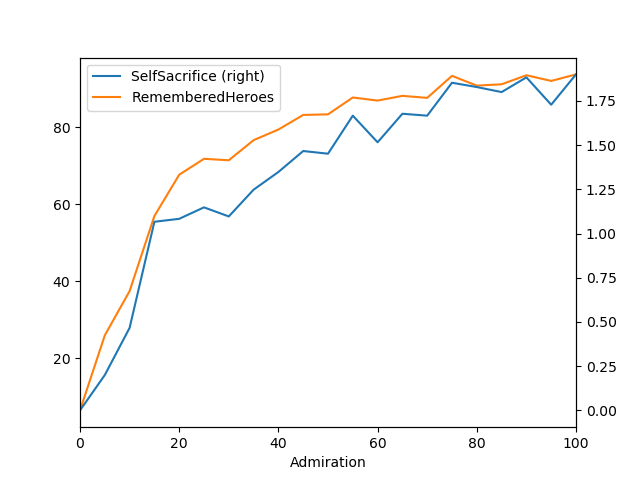
\includegraphics[width=1\textwidth]{RGT_10}
\caption{$\bf{SelfSacrifice}$ and $\bf{RememberedHeroes}$, as a function of \emph{Admiration} (typical parameter values).}
\label{fig:RGT_10}
\end{figure}



\textbf{Figure \ref{fig:RGT_10}} shows results obtained by averaging over 30 simulations, according to the \emph{Admiration}
 parameter (all others being kept constant at the previously described values). As could be expected, $\bf{RememberedHeroes}$
 rises from 0 with \emph{Admiration}, quickly reaching two thirds of its maximum value of under 100 heroes when
 \emph{Admiration} exceeds 20. 
 
 $\bf{SelfSacrifice}$ follows similar dynamics, with values ranging between 0 and 2\% (values to a higher precision than
 the percentage point being obtained artificially by averaging over experimental results). These values are far from negligible:
 for a typical population of 200, we expect an average of (almost) 4 martyrs each year.
 Such collective behavior is captured here by individuals all bearing similar genetic probability $P$
 of self-sacrifice at equilibrium (and obtaining similar $\bf{Reproductive\_points}$ in the 
 long-term), as seen on \textbf{Figure \ref{fig:Snap}}. 
 
 \begin{figure}[h]
    \centering
    \begin{subfigure}[b]{0.3\linewidth} 
        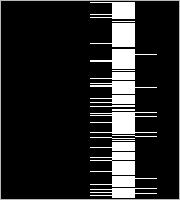
\includegraphics[width=\linewidth, height =\linewidth]{Exo_Genome}
        \caption{Genetic values}
    \end{subfigure}
    \begin{subfigure}[b]{0.3\linewidth}
        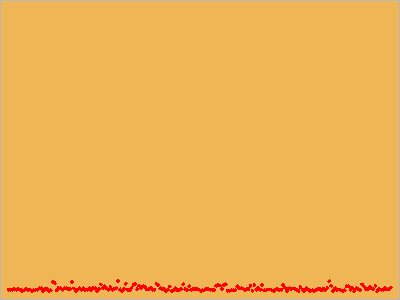
\includegraphics[width=\linewidth, height = \linewidth]{Exo_Field}
        \caption{Reproductive points}
    \end{subfigure}
    \caption{Snapshot of individual values, \emph{A=50}. An individual's genome is represented by a horizontal line on the left: here most bear a $\bf{SelfSacrifice}$ gene
    of relative value $\frac{2^2}{2^8-1}$ (around $1.6\%$). Individuals (horizontal axis) and their reproductive points (vertical) are represented on the right.}
    \label{fig:Snap}
    \end{figure}


 However, one can also imagine the collectively equivalent situation where only a small fraction $f$ of individuals
 engage in self-sacrificial behavior with higher probability $p$ (with $P = f*p$), to the much more
 significant benefit of their families (see \textbf{Section \ref{sec_exo_math}}).

\subsection{Influence of \emph{ReproGainsThreshold} $RGT$}

\begin{figure}[h]
    \centering
    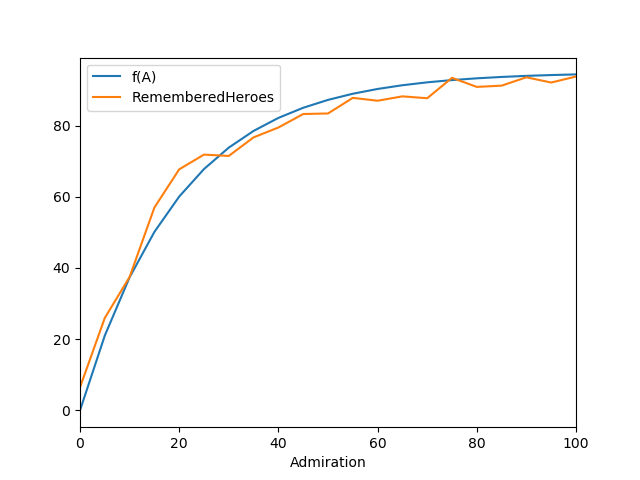
\includegraphics[width=0.6\textwidth]{f_rgt10}
    \caption{$\bf{RememberedHeroes}$ and corresponding optimal $f$ as functions of 
    \emph{Admiration}, for $RGT=10$ ($C=95, \tau = 20$).}
    \label{fig:f_10}
    \end{figure}

As a function of \emph{Admiration}, $\bf{RememberedHeroes}$ resembles a function of the form:
$f_{C,\tau}(t) = C*(1-exp(-t/\tau))$.
% Com sur la forme de la fonction ? Par ex: selection d'une allele, cf Nettle p80
% ou radioactive decay / pop growth with ...
Very approximately\footnote{By choosing optimal C and $\tau$ at a precision of 5 units;
the idea here being simply to get a "feel" for overall variation with $A$. Optimal parameters are the
ones for which Euclidean distance is minimal.},
it can best be approached by a function of this form with parameters $C=95$ and $\tau = 20$, as visible
on \textbf{Figure \ref{fig:f_10}}.

\begin{figure}[h]
    \centering
    \begin{subfigure}[b]{0.4\linewidth} 
        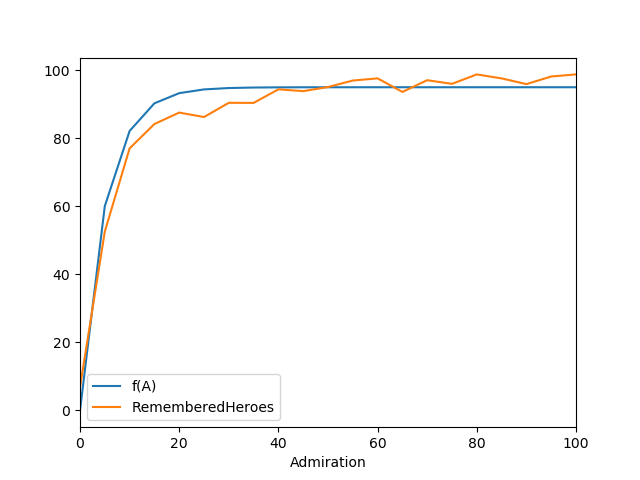
\includegraphics[width=\linewidth]{f_rgt5}
        \caption{$RGT=5$ ($C=95,\tau=5$)}
    \end{subfigure}
    \begin{subfigure}[b]{0.4\linewidth}
        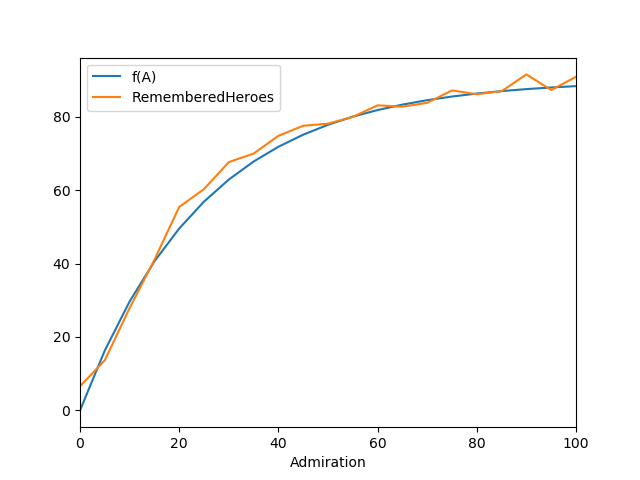
\includegraphics[width=\linewidth]{f_rgt20}
        \caption{$RGT=20$ ($C=90,\tau=25$)}
    \end{subfigure}
    \caption{$\bf{RememberedHeroes}$ and $f$ for $RGT=5, 20$}
    \label{fig:RGT5-20}
    \end{figure}

The key parameter governing relative growth of $\bf{RememberedHeroes}$\footnote{
This output's absolute value is arbitrary, chosen according to \emph{RemThreshold} in
order to provide for visible variations (see \textbf{Section \ref{ss:RH}}).
} thus appears to be one equal to two times
\emph{ReproGainsThreshold}. The importance of $RGT$ is not surprising since it plays
the crucial role of defining the unit in which $\bf{Reproductive\_points}$ are counted.  
The relationship between $RGT$ and final results is however non-trivial, since 
variation according to $A$ for $RGT=5$ (resp. $RGT=20$) are best captured by $\tau=5$
(resp. $\tau=25$), as visible on \textbf{Figure \ref{fig:RGT5-20}}; suggesting perhaps
a quadratic relationship between $RGT$ and $\tau$. \textbf{Section \ref{ss: exo_existence}}
returns to this issue.
%%% A MODIF : provides a charac for minimal ESS > 0... et plus si affinites?

\subsection{Variation with \emph{SacrificeHeredity} $h$}

%%% Au moins le graphe A = 50 vs h... => et donc ?
Contrary to what could be expected, h -> 1 is a problem: probs because pop = too small
and all end up with same h... - as shown by simu // because same family ? (or just expected in LT?)
h = 0 discontinuity = expected

\subsection{Variation with \emph{ReproductionRate} $r$}
%%% Duh, with N... // and also relationship p and r visibly => cf section 1.3.3.

\section{Exogenous model: mathematical proof of concept}
\label{sec_exo_math}
%%% BONUS : here add f << 1 : using equation on A * ... / f < RGT...

\subsection{Simplifying assumptions and characterization of equilibrium}
\label{ss:exm_eq}
Individuals live to a maximum of \emph{AgeMax} $M$ years, fixed at 40 here. 
 Expected life span is lower however, as individuals face random accidents
 (in a wide sense) and is equal to $\alpha*M$, where $\alpha$ captures
 the effects of natural selection. In this model, all individuals face the same $\alpha$, but
 may obtain differing reproductive opportunities ($\bf{Selectivity}$ mode).

An individual who engages in self-sacrificial behavior with probability $p$
 shortens his/her expected lifespan by a multiplicative factor of (see \textbf{Appedix \ref{beta}}):
 
\begin{equation}
 \beta(p) = \frac{(1-p) - (1-p)^{(M+1)}}{p*M} 
\label{eq_beta}
\end{equation}

As such, said individual's reproductive window is shorter, which should lead to the disappearance of
 self-sacrificial behavior - unless this is compensated by increased reproductive opportunities. In contrast to how the
 actual simulation is played, let us assume that: 
 \begin{itemize}
\item Only a \textit{negligible proportion $f$} of individuals engage in self-sacrificial behavior, with equal probability $p$;
\item These future "heroes" will be the first this society sees (everyone starts off with no $\bf{Reproductive\_points}$ $RP$);
\item Generations do not overlap;
\item Individuals are granted their lifetime reproductive potential $R$ at birth
(in contrast with a year-by-year attribution).
\end{itemize}
 
In such a situation, individuals who engage in self-sacrificial behavior obtain on average $\alpha*\beta(p)*M*r$ offspring, 
with others obtaining $\alpha*M*r$, where $r$ is the population-level \emph{ReproductionRate}. However,
the former's children are granted a larger reproduction potential $R_+(A,f)$, which notably
depends on \emph{Admiration} $A$. Since $f$ is assumed to be very small, $R_+(A,f)$ is the same for all
children of individuals who self-sacrifice (we neglect the possibility of individuals being born from two
would-be martyrs), and the children of non-would-be martyrs obtain a reproductive potential which can be
approximated to $r$.

If, in addition, we assume that \emph{$p$ and $M$ are sufficiently large}\footnote{We still expect
$P=f*p$ to be relatively small, to avoid "martyr over-crowding",
but for this to be primarily due to $f$, in the current mathematical characterization.}
for would-be heroes to largely end up
actually laying their life for the group (and not dying in another way), such individuals obtain 
on average $R_+(A,f)*\alpha*\beta(p)*M*r$ grand-children, 
while others obtain $\alpha*M*r^2$. Thus, a first-order
\footnote{Note that apart from (\ref{eq:min_ESS_e}) equations in this section are valid at best at the
first-order in $f<<1$ and are computed for expected values.}
(neglecting the effects on subsequent generations) characterization of equivalence between both strategies can be written as:
%p and M large debatable ?? Not that much, maybe add a note /// add that we still expect P to be small
 
\begin{equation}
    R_+(A,f)*\beta(p) = r
\label{eq:grandchildren}
\end{equation}
%% le environ egal devient egal...

%%%% POURQUOI JLD VOULAIT RAJOUTER DES f???

\subsection{Necessary condition for an ESS}
\label{ss: exo_existence}

Let $N$ be equal to \emph{PopulationSize}, implicitly assumed to be large here (since $f$
is negligible).

In the spirit of the simplifying assumptions made above, let us assume
that total social admiration is borne the children of non-heroes, and is thus equal to
$A*(1-f)N*\alpha Mr$. For children of martyrs, two cases are possible:

\begin{itemize}
\item either $\frac{A*(1-f)N*\alpha Mr}{fN*\alpha\beta(p)Mr} < RGT$, and 
all receive reproductive potential $r$;
\item or $\frac{A*(1-f)N*\alpha Mr}{fN*\alpha\beta(p)Mr} \geq RGT$, and all receive $R_{+}(A,f)>r$.
\end{itemize}

Thus, (p,f) can only constitute an ESS if:

\begin{equation}
    \label{eq:min_ESS_e}
    A \geq A_{min}=\frac{RGT*f*\beta(p)}{1-f}  
    \iff f \leq f_{max} = \frac{A}{RGT*\beta(p)+A}
\end{equation}
%ca existe tjs un ESS ? Pas sur, c'est plutot l'eq de Nash en strat mixte...


%%% POUBELLE : version ou l'admiration vient des parents: change pas grand chose en vrai...

%Following the simplifying assumptions made above, total social admiration is
%borne from each non-hero in the first generation and is thus equal to $A*N*(1-P)$.
%For children
%of martyrs, two cases are possible (on average):

%\begin{itemize}
%\item either $\frac{AN(1-P)}{fN*\alpha\beta(p)Mr} < RGT$, and each receives reproductive potential $r$;
%\item or $\frac{AN(1-P)}{fN*\alpha\beta(p)Mr} \geq RGT$, and each receives $R_{+}(A,f)>r$.
%\end{itemize}

%Since, in our simplified model, unchecked population growth from one generation to the next
%is equal to a factor of $Mr$\footnote{Rather than $(1+r)^M$ over M years}, we can assume
%that, at equilibrium, natural selection compensates such growth: $\alpha = \frac{1}{Mr}$.

%Thus, (p,f) can only constitute an ESS if:

%\begin{equation}
%    \label{eq:min_ESS_e}
%    A \geq A_{min}=\frac{RGT*f*\beta(p)}{1-p*f}  
%    \iff f \leq f_{max} = \frac{A}{RGT*\beta(p)+p*A}
%\end{equation}
%ca existe tjs un ESS ? Pas sur, c'est plutot l'eq de Nash en strat mixte...


%In a population composed of $N-1$ non-heroes and one mutant would-be martyr, the latter will
%thus be able to invade if, in particular\footnote{ $\alpha$ and $\beta(p)$ are smaller than 1.}:

%\begin{equation}
%    A > A_{min} = \frac{RGT*M*r}{N} 
%\label{eq:ESS}
%\end{equation}


% on obtient p = 9,3% avec nos valeurs... (which is not too small) /// [and P = p/200 = 0.004] ///
%OK really smally f if you take N big...

% ici mettre la figure pour Beta en fait... ?




%%% BONUS : here add f << 1 : using equation on A * ... / f < RGT...
%\section{A posteriori justification of $f<<1$}
% ca marche ca ???
%% si condition sur f => condition sur P avec le p d'en-dessous

\subsection{Mathematical characterization of the ESS}

%%% COMMENCER ICI / dans l'annexe correspondante : calcul de p a l'eq... (sachant f petit...)
%% => pb pour l'AN ???


As shown in \textbf{Appendix \ref{ss:R+}}, a first-order approximation of $R_+$
in the latter case is ($S$ is equal to \emph{Selectivity}):
\begin{equation}
    R_+(A,f) = \frac{S*r}{log(1+S)} * (1 - \frac{f*\beta(p)}{2})
\label{eq:R+}
\end{equation}

This allows us to deduce first-order approximations for $\beta(p)$ and $p$ at (potential) ESS, as shown in
\textbf{Appendix \ref{ss_e_a:ESS}}:

\begin{equation}
    \label{eq:ESS_e_duh_beta}
    \beta(p) = \frac{r}{R_{max}}+\frac{1}{2}*(\frac{r}{R_{max}})^2*f
\end{equation}

 \begin{equation}
    \label{eq:approx_p_exo}
    p(S,M,f) = \frac{1}{1+M*\frac{log(1+S)}{S}}*
    (1- \frac{\frac{1}{2}*
    (\frac{log(1+S)}{S})^2}{1+M*\frac{log(1+S)}{S}})*f
    \end{equation}



%%% ++ Pourquoi je mets ces equations ?? Elles n'apportent pas grand chose 
%au final... 

Using (\ref{eq:min_ESS_e}), we also deduce that, for such an ESS to exist, we must have:
\begin{equation}
    \label{eq:min_A_e}
    A \geq A_{min}(RGT,S,f)=\frac{RGT*log(1+S)}{S}*f
\end{equation}

%%% A VIRER ! / contraire a l'autre equation...
%\begin{equation}
  %  \label{eq:max_f_e}
  %  f \leq f_{max} = \frac{A*S}{RGT*log(1+S)+A*S}
%\end{equation}



%Using (\ref{eq:min_ESS_e}), we deduce that, for such an ESS to exist, we must have:
%\begin{equation}
 %   \label{eq:min_A_e}
  %  A \geq A_{min}=\frac{RGT*f*log(1+S)}{S*(1-f)}  
%\end{equation}

%\begin{equation}
 %   \label{eq:max_f_e}
  %  f \leq f_{max} = \frac{A*S}{RGT*log(1+S)+A*S}
%\end{equation}
%
%\begin{figure}[h]
 %   \centering
  %  \begin{subfigure}[b]{0.4\linewidth} 
   %     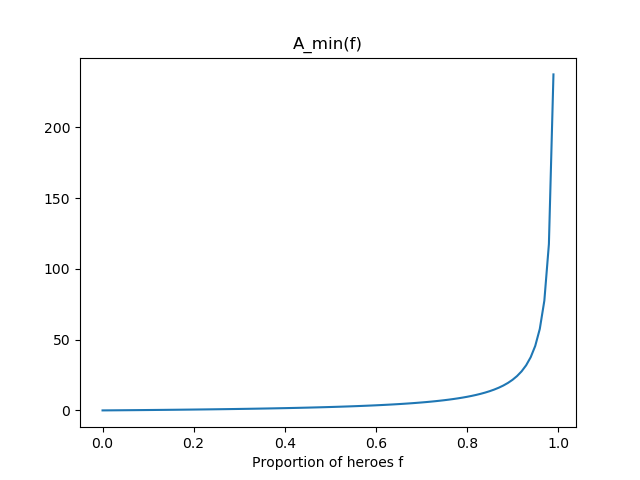
\includegraphics[width=\linewidth]{A_min}
    %    \caption{$A_{min}(f)$}
%    \end{subfigure}
 %   \begin{subfigure}[b]{0.4\linewidth}
  %      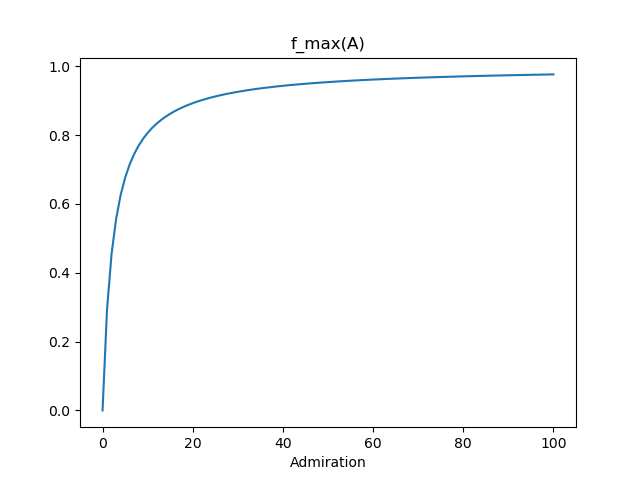
\includegraphics[width=\linewidth]{f_max}
   %     \caption{$f_{max}(A)$}
    %\end{subfigure}
%    \caption{Boundary conditions (typical parameters)}
 %   \label{fig:A_f_m}
  %  \end{figure}


% = SUBSECTION actually ?
\subsection{Brief Discussion}
% PoC x2 avec la simu aussi...

% // ou relationship with before...
p = + function of S = duh // - of M : more to sacrifice
But \textbf{no r}, no A
% CAR bizarre de mettre r dans nb enfants heros ???? --> a l'eq part deja de R+... ?
% oui mais reviendrait au meme dans calcul je pense...
$---> should be captured by f.... : OK for A in f_max...$
Maybe cheat : admiration goes to heroes = the parents... then to children ? How ?
= need to have a generational gap (but cool here that f between 0 and 1)


+ RGT : here = linear law... probs because of approx f<<1, all receive the same\dots

+ h: not here, vu le modele



+ lim for JLD : does not depend on nb of heroes... -> visibility log(nbheroes... ?)

%When \emph{Admiration} is sufficient large, self-sacrifice with overall probability $P=f*p$ is thus an ESS
%when $p$ and $f$ verify:




%% le environ egal devient egal...


% bon en vrai y a pas de r, mais on voit l'idee.... RGT gouverne bien le truc : cf les graphes...
% this = really extreme, but then again N*r is not that big...

%% PB : comment ramener le f ???


%MATH + => demo that small proba + ... + ...


% on obtient p = 9,3% avec nos valeurs... (which is not too small) /// [and P = p/200 = 0.004] ///
%OK really smally f if you take N big...

% ici mettre la figure pour Beta en fait... ?




%%% BONUS : here add f << 1 : using equation on A * ... / f < RGT...
%\section{A posteriori justification of $f<<1$}
% ca marche ca ???
%% si condition sur f => condition sur P avec le p d'en-dessous















\section{"Endogenous" model}
%/actual model...

\subsection{Simulation outputs}

\subsection{Mathematical analysis}

salut
\ref{eq:grandchildren}



\section{Limitations}
%Oops NonPatriots that actually self-sacrifice....
%% HERE MORE LIKE ?

\chapter{Perspectives}
%%\section{Limitations}
%Oops NonPatriots that actually self-sacrifice....

%\part*{Bibliography}
%take out III ?
%\bibliographystyle{plain}
%\bibliography{/home/tom/Documents/Stage/Memoire/Memoire}

%\cite{dessalles_optimal_2014}
\bibliographystyle{apacite}
\bibliography{Memoire}
%%%%%%%%%%%%%%% oops url too long...

\appendix
%\part{Appendix}
%Take out IV?

\chapter{Python stuff}
\label{a:scripts}
\chapter{Mathematical demonstrations}

\section{Exogenous model}
\subsection{RemTH}
\subsection{$\beta(p)$}
\label{beta}

Disregarding the effects of natural selection (which are the same for all individuals 
here\footnote{And will therefore appear on both sides of an equation comparing
the benefits of either strategy such as (\ref{eq:grandchildren}).}),
 an individual who bears a $\bf{SelfSacrifice}$ gene of relative value $p$, has a probability $p$ of dying in his first year
 (before being able to foster any descendants), a probability $(1-p)*p$ of dying at age $1$ ...
 a probability $(1-p)^{n}*p$ of dying at age $n<M$ ... and is certain to die at age $M$, should
 he or she reach it. His/her expected life span is thus:

 \[ ELS = p*0 + (1-p)*p*1 + ... + (1-p)^{M-1}*(M-1) + (1-p)^M*M \]

Let $f \colon \mathbf{R} \to \mathbf{R}$ be the polynomial function defined by the expression:
\[ f(x) = \sum_{n=0}^{M-1} p*(1-p)^n*x^n + (1-p)^M*x^M \]

By deriving $f$, one can note that:
\begin{equation}
    ELS = f'(1)
\label{eq_ELS_f}
\end{equation}

$f(x)$ involves a geometric sum and can be simplified to (when $(1-p)*x$ is different than 1):

\[ f(x) = p* \frac{1 - ((1-p)*x)^M}{1-(1-p)*x} + ((1-p)*x)^M \]

For $x\neq\frac{1}{(1-p)}$ ($p=1$ trivially yields $ELS=0$):

\[ f'(x) = p * \frac{-M(1-p)^Mx^{M-1}*(1-(1-p)x) + (1-p)*(1-((1-p)x)^M)}{(1-(1-p)x)^2} + M(1-p)^Mx^{M-1} \]

And thus:

\[f'(1) = p * \frac{(-M(1-p)^M*p + (1-p)*(1-(1-p)^M)}{p^2} + M(1-p)^M \]

\begin{equation}
    f'(1) = \frac{(1-p)*(1-(1-p)^M)}{p}
\label{eq_f'}
\end{equation}

Combining these two expressions for $f'(1)$ proves equation ($\bf\ref{eq_beta}$). \textbf{Figure \ref{fig:beta}} shows
$\beta(p)$ for $p$ between 0 and 1. Factoring in natural selection, an individual's expected life span is therefore equal to: $\alpha*\beta(p)*M$.

\begin{figure}[h]
    \centering
    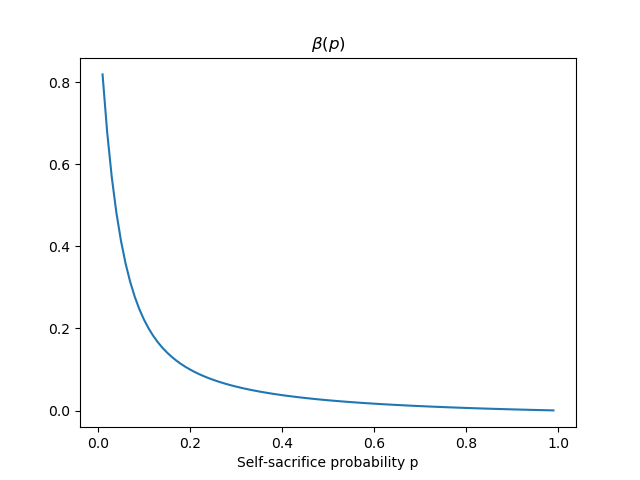
\includegraphics[width=1\textwidth]{Beta}
    \caption{Loss of expected life-span due to self-sacrifice.}
    \label{fig:beta}
    \end{figure}
    



\subsection{$R_{+}(A)$}
\label{ss:R+}
In $\bf{Selectivity}$ mode, individuals obtain reproductive potential $R$ according to their
$\bf{Reproductive\_points}$ $RP$, each individual obtains a rank $k$
according to $RP$, and receives reproductive potential:
\[ R = \frac{r}{2} * (\frac{S}
{(S*k + N')*log(1+S)} + \frac{S}{(S*(k+1) + N')*log(1+S)}*N') \]

where $N'<N$ is the number of eligible parents (non-martyrs) and $S$ is equal to \emph{Selectivity}
(the average reproductive potential over eligible parents being \emph{ReproductionRate} $r$).
When $N >> 1$, $R$ verifies:

\begin{equation}
    R \in [R_{min};R_{max}], \textrm{with } R_{max} \approx \frac{S*r}{log(1+S)} 
    \textrm{ and } R_{min} \approx
    \frac{R_{max}}{1+S}
\label{eq:ReproPot}
\end{equation}

With typical parameters ($S=10$ and $r=15\%$), we obtain: $R_{max} \approx 63 \%$ and 
$R_{min} \approx 5,6 \%$.

In a case where a negligible proportion $f$ of individuals engage in
self-sacrificial behavior (which is assured to end up in their martyrdom), their children each
receive, on average:
\begin{itemize}
\item reproductive potential $r$, when $\frac{AN(1-P)}{fN*\alpha\beta(p)Mr} < RGT$;
\item $R_{+}(A,f)$ otherwise, as seen in \textbf{Section \ref{ss: exo_existence}}.
\end{itemize}

When $N>>1$, expected $R_+(A,f)$ is equal to the average between the "luckiest" ($k=0$) and "unluckiest"
child, which is approximately:
\[ R_+(A,f) \approx \frac{S*r}{2*log(1+S)} * (1 + \frac{N'}{S*fN*\alpha\beta(p)Mr+N'})\]

\[ R_+(A,f) \approx \frac{S*r}{2*log(1+S)} * (1 + \frac{1}{\frac{S*fN*\alpha\beta(p)Mr}{(1-f)N*\alpha Mr + fN*\alpha\beta(p)Mr}+1})\]

\[ R_+(A,f) \approx \frac{S*r}{2*log(1+S)} * (1 + \frac{(1-f) + f\beta(p)}{(S+1)*f*\beta(p)+(1-f)})\]

Which yields, for $f<<1$ (neglecting terms of order 2 and above):

\begin{equation}
    \tag{\ref{eq:R+}}
    R_+(A,f) \approx  \frac{S*r}{log(1+S)} * (1 - \frac{f*\beta(p)}{2}) = R_{max}*(1-\frac{f*\beta(p)}{2})
\end{equation}

\subsection{ESS}
\label{ss_e_a:ESS}

Using (\ref{eq:grandchildren}), we deduce that both envisioned strategies are equivalent if
and only if (at this level of approximation):

\[\frac{Sr}{log(1+S)}(1-\frac{f\beta(p)}{2})\beta(p)=r  \]

\begin{equation}
    \label{eq:trinome_beta}
    \iff f*\beta(p)^2 - 2*\beta(p) + 2*\frac{r}{R_{max}} = 0
\end{equation}

This is a quadratric equation in $\beta(p)$, whose reduced discriminant $\delta$ verifies:

\[\delta = 1 - 2f\frac{r}{R_{max}} > 0 \textnormal{ since } 
r<R_{max} \textnormal{ and } f << 1 
\]

Since $\beta(p)$ is smaller than 1, the
only possible solution is:

\[\beta(p) = \frac{1 - \sqrt{1-\frac{2fr}{R_{max}}}}{f} \]

Yielding, for $f << 1$:

\begin{equation}\tag{\ref{eq:ESS_e_duh_beta}}
    \beta(p) = \frac{r}{R_{max}}+\frac{1}{2}*(\frac{r}{R_{max}})^2*f
\end{equation}

%Un peu con: equivalent a faire une approx violente avec tlm a Rmax ?
%% ===> RAISONNEMENT TROP COMPLIQUE, il doit y avoir une maniere plus simple

Since $\beta \colon [0,1] \to [0,1]$ is a bijection, as visible on
 \textbf{Figure \ref{fig:beta}}, 
 this yields a unique $p(f)$ = $\beta^{-1}(\frac{log(1+S}{S} + \frac{1}{2}(\frac{log(1+S)}{S})^2f)$
 for a given $f$. With typical parameter values, and $f\leq 1\%$
 we find $p \approx 9.3\%$, by zeroing in on p at a precision of .1\%.

 In addition, if we suppose that $(1-p)^{M+1} << (1-p)$, which is the case here, then we
 can calculate an approximation\footnote{Which would have yielded
 $p \approx 9.4\%$.} for $p$:

 \[p \approx \frac{1}{1+M*(\frac{log(1+S)}{S} + \frac{1}{2}*(\frac{log(1+S)}{S})^2*f)}\]


 \begin{equation}
    \tag{\ref{eq:approx_p_exo}b}
    p \approx \frac{1}{1+M*\frac{log(1+S)}{S}}*
    (1- \frac{\frac{1}{2}*
    (\frac{log(1+S)}{S})^2}{1+M*\frac{log(1+S)}{S}})*f
    \label{eq:p_grr_approx}
    \end{equation}


% \begin{equation}
 %   \tag{\ref{eq:approx_p_exo}b}
  %  p \approx \frac{S}{M*log(1+S)+S}
 %\end{equation}

 In a potential self-sacrifice ESS involving a negligible proportion $f$ of agents that lay down their
 life with probability $p$, then $p$ can be thus approximated.


 
\end{document}

%Tous les calculs sont faits en moyenne / esperance... pas precise a chaque fois ?


%Using (\ref{eq:min_ESS_e}), we can further deduce that for such an ESS to exist,
%we must have:

%\[A \geq A_{min}=\frac{RGT*f*log(1+S)*(M*log(1+S)+S)}{(M*log(1+S)+S)*S - S^2*f}  \]
    
%\[f \leq f_{max} = \frac{A*S(M*log(1+S)+S)}{RGT*log(1+S)+S*A}\]
